\documentclass{beamer}

\usepackage{amsmath, amsthm, amssymb, mathtools}

\usepackage{graphicx}
\graphicspath{ {./images/} }

\usepackage{pgfplots}
\pgfplotsset{width=12cm,height=8cm,compat=1.18}
\usepgfplotslibrary{fillbetween}
\usepgfplotslibrary{external}
\usetikzlibrary{patterns}

\usetikzlibrary{external}
\tikzexternalize[
   mode=list and make,
   figure list=true,
   prefix=figures/
]

\usetheme{JuanLesPins}
\usecolortheme{default}

\Umathopinnerspacing\displaystyle=0mu
\Umathopinnerspacing\textstyle=0mu

\begin{document}

\title{Bisection Method}
\subtitle{Mathematics for AI I, KO}
\author[]{Yevhenii Konyshev}

\date{\today}

\frame{\titlepage}

\begin{frame}
    \frametitle{Table of contents}

    \tableofcontents
\end{frame}

\AtBeginSection[]
{
    \begin{frame}<beamer>
        \frametitle{Outline}
        \tableofcontents[currentsection]
    \end{frame}
}

\section{Definition of a Continuous Function}

\begin{frame}
    \frametitle{Definition of a continuous function}

    Let's begin with the most essential idea: the definition of a continuous function which we need to discuss as the intermediate value theorem, on which the bisection method is based, is defined for continuous functions.
\end{frame}

\begin{frame}
    \frametitle{Definition of a continuous function}

    \begin{definition}[Continuous function]
        Let $D \subset \mathbb{R}$ and $f \colon A \to B$. \\
        $f$ is \textbf{continuous} if and only if
        for all $x \in D$, for all $\left(x_n\right)_{n \in \mathbb{N}}$ with $x_n \to x$ we have that

        $$\lim_{n \to \infty}{f(x_n)} \text{ exists } \wedge \lim_{n \to \infty}{f(x_n)} = f(x) = f\left(\lim_{n \to \infty}{x_n}\right)$$
    \end{definition}
\end{frame}

\section{Definition of the Intermediate Value Threorem (IVT)}

\begin{frame}
    \frametitle{Definition of the Intermediate Value Theorem (IVT)}

    Now that we have defined the notion of a continuous function we may talk about an important property of continuous functions: the intermediate value theorem. \\~\
\end{frame}

\begin{frame}
    \frametitle{Definition of the Intermediate Value Theorem (IVT)}

    \begin{theorem}[Intermediate value theorem]
        Let $I = \left[a, b\right]$ and $f \colon I \to \mathbb{R}$ be a continuous function. \\
        Then, for all $y \in \mathbb{R}$ with
        $$\min{\left\{f(a), f(b)\right\}} \leq y \leq \max{\left\{f(a), f(b)\right\}}$$
        we have that $$\exists x \in I \colon f(x) = y.$$
    \end{theorem}
\end{frame}

\begin{frame}
    \frametitle{Understanding the intermediate value theorem}

    The theorem can also be interpreted as every value between $f(a)$ and $f(b)$ being attained by the continuous function $f$. \\~\

    More precisely, the image of the bounded interval $[a, b]$ under $f$ is a superset of the bounded interval defined by $f(a)$ and $f(b)$.
    $$f([a, b]) \supset \left[\min{\left\{f(a), f(b)\right\}}, \max{\left\{f(a), f(b)\right\}}\right]$$
\end{frame}

\section{Proof of the Intermediate Value Threorem (IVT)}

\begin{frame}
    \frametitle{Proof of the IVT}

    To get an idea how one could compute the value of $x$ by exploiting the continuity of $f$ let's have a closer look at the proof of the intermediate value theorem.
\end{frame}

\begin{frame}
    \frametitle{Proof of the IVT}

    \begin{block}{Proof.}
        Case 1: $f(a) = f(b)$:

        $\min{\left\{f(a), f(b)\right\}} \leq y \leq \max{\left\{f(a), f(b)\right\}}, f(a) = f(b)$ \\
        $\implies y = f(a) = f(b)$ \\
        Pick $x = a = b \implies f(x) = y$.

        \vspace{5mm}

        Case 2: $f(a) \neq f(b)$:

        The case $f(a) > f(b)$ can be proven the same as $f(a) < f(b)$ by replacing $f$ with $-f$, where $-f(a) < -f(b) \iff f(a) > f(b)$
        and looking for $x$ with $-y = -f(x) \iff y = f(x)$, so we can assume w.l.o.g. that $f(a) < f(b)$.
    \end{block}
\end{frame}

\begin{frame}
    \frametitle{Proof of the IVT}

    \begin{block}{Proof. (Cont.)}
        As we consider a function $f$ defined on a closed interval $[a, b] \neq \varnothing$, we have $a \leq b$.

        \vspace{2.5mm}

        Now let $y, \min{\left\{f(a), f(b)\right\}} \leq y \leq \max{\left\{f(a), f(b)\right\}}$ $\implies y \in [f(a), f(b)]$ a.b.f, 

        \vspace{2.5mm}

        We define $(m_n)_{n \in \mathbb{N}}$ with $m_n \to x \in I$ and $f(x) = y$.

        First of all, let $a_0 \coloneq a, b_0 \coloneq b$ and $m_0 \coloneq \frac{a_0 + b_0}{2}$, i.e., the $m_0$ is the midpoint between $a_0$ and $b_0$, and also we define

        $$
        a_1 \coloneq \begin{cases}
            m_0, & f(m_0) < y \\
            a_0, & f(m_0) \geq y
        \end{cases}
        $$
    \end{block}
\end{frame}

\begin{frame}
    \frametitle{Proof of the IVT}

    \begin{block}{Proof. (Cont.)}
        $$
        b_1 \coloneq \begin{cases}
            b_0, & f(m_0) < y \\
            m_0, & f(m_0) \geq y
        \end{cases}
        $$

        $$m_1 \coloneq \frac{a_1 + b_1}{2}$$
        For $a_1$ and $b_1$ it holds that $a_0 \leq a_1 < \ldots < b_1 \leq b_0$ and $f(a_1) \leq y \leq f(b_1)$,
        moreover, $b_1 - a_1 = \frac{b_0 - a_0}{2}$.
    \end{block}
\end{frame}

\begin{frame}
    \frametitle{Proof of the IVT}

    \begin{block}{Proof. (Cont.)}
        Let $n \in \mathbb{N}_0$ a.b.f. and we generalize the above definitions

        $$a_0 \coloneq a,\,b_0 \coloneq b$$

        $$
        a_{n + 1} \coloneq \begin{cases}
            m_n, & f(m_n) < y \\
            a_n, & f(m_n) \geq y
        \end{cases}
        $$

        $$
        b_{n + 1} \coloneq \begin{cases}
            b_n, & f(m_n) < y \\
            m_n, & f(m_n) \geq y
        \end{cases}
        $$

        $$m_n \coloneq \frac{a_n + b_n}{2}$$
    \end{block}
\end{frame}

\begin{frame}
    \frametitle{Proof of the IVT}

    \begin{block}{Proof. (Cont.)}
        With this we can define two sequences: $(a_n)_{n \in \mathbb{N}}$ and $(b_n)_{n \in \mathbb{N}}$ with

        \begin{equation}
            \label{mon}
            a = a_0 \leq a_1 \leq \ldots \leq a_n < \ldots < b_n \leq \ldots \leq b_1 \leq b_0 = b
        \end{equation}

        i.e, the sequences are monotone and bounded $\implies$ convergent by the monotonicity principle. \\~\

        We also show that $m_n$ is contained within $[a_n, b_n]$, i.e. $a_n < m_n < b_n$.
    \end{block}
\end{frame}

\begin{frame}
    \frametitle{Proof of the IVT}
    \begin{block}{Proof. (Cont.)}
        $$a_n < b_n \iff b_n - a_n > 0 \iff \frac{b_n - a_n}{2} > 0$$
        $$m_n = \frac{a_n + b_n}{2} = \frac{2a_n + b_n - a_n}{2} = a_n + \frac{b_n - a_n}{2} > a_n$$
        $$a_n < b_n \iff a_n - b_n < 0 \iff \frac{a_n - b_n}{2} < 0$$
        $$m_n = \frac{a_n + b_n}{2} = \frac{2b_n + a_n - b_n}{2} = b_n + \frac{a_n - b_n}{2} < b_n$$

        \begin{equation}
            \label{middle_bounds}
            a_n < m_n < b_n
        \end{equation}
    \end{block}
\end{frame}

\begin{frame}
    \frametitle{Proof of the IVT}

    \begin{block}{Proof. (Cont.)}
        Also, $b_n - a_n = \frac{b - a}{2^n} \to 0$ as $n \to \infty$,
        therefore, $\displaystyle\lim_{n \to \infty}{a_n} = \lim_{n \to \infty}{b_n}$, we define $x$ in the follwing manner:

        \begin{equation}
            \label{limits}
            \lim_{n \to \infty}{a_n} = \lim_{n \to \infty}{b_n} \eqqcolon x \in [a, b]
        \end{equation}

        and prove $f(x) = y$ next. \\~\

        We also have that $m_n \to x$ as $n \to \infty$ by the sandwich rule considering (\ref{mon}) combined with (\ref{middle_bounds}), and (\ref{limits}).
    \end{block}
\end{frame}

\begin{frame}
    \frametitle{Proof of the IVT}

    \begin{block}{Proof. (Cont.)}
        Second of all, from $f(a_n) \leq y \leq f(b_n)$ we have
        $$\lim_{n \to \infty}{f(a_n)} \leq \lim_{n \to \infty}{y} \leq \lim_{n \to \infty}{f(b_n)}$$

        $y$ is constant w.r.t. $n$, hence

        \begin{equation}
            \label{bounded}
            \lim_{n \to \infty}{f(a_n)} \leq\ y \leq \lim_{n \to \infty}{f(b_n)}
        \end{equation}
    \end{block}
\end{frame}

\begin{frame}
    \frametitle{Proof of the IVT}

    \begin{block}{Proof. (Cont.)}
        Using the continuity of $f$ and also (\ref{limits}) we obtain
        $$f(x) \overset{(\ref{limits})}{=} f\mathopen{}\left(\lim_{n \to \infty}{a_n}\mathclose{}\right) \overset{f \text{ is cont.}}{=} \lim_{n \to \infty}{f(a_n)} \overset{(\ref{bounded})}{\leq} y$$
        $$y \overset{(\ref{bounded})}{\leq} \lim_{n \to \infty}{f(b_n)} \overset{f \text{ is cont.}}{=} f\mathopen{}\left(\lim_{n \to \infty}{b_n}\mathclose{}\right) \overset{(\ref{limits})}{=} f(x)$$

        $$f(x) \leq y \leq f(x) \iff f(x) = y$$
        \qed
    \end{block}
\end{frame}

\section{High-level Summary of the Proof}

\begin{frame}
    The most important part is how the sequences $(a_n)$ and $(b_n)$ are defined.
    Granting convergence by the monotonicity principle, moreover, convergence to 
    the same number we define as $x$ as the distance between the elements is $0$ at $\infty$. \\~\

    And we investigate this part of the proof with some visualizations.
\end{frame}

\begin{frame}
    \frametitle{High-level summary of the proof and the basis for the algorithm}

    For our particular case of $f(a) < f(b)$ the general principle by which $(a_n)$ and $(b_n)$ were constructed is as follows: \\~\

    If $f(m_n) \geq y$, i.e., the value of $f$ at the middle of $[a_n, b_n]$ is greater than $y = f(x)$ and, conversely,
    thanks to the continuity of $f$, we can assume $m_n \geq x$, therefore, picking $a_{n + 1} = a_{n}$, $b_{n + 1} = m_n$, which still preseves the main property: $f(a_{n + 1}) < y < f(b_{n + 1})$. \\~\

    The $[a_{n + 1}, b_{n + 1}] = [a_n, m_n] \subset [a_n, b_n]$ becomes the `left half' of $[a_n, b_n]$.
\end{frame}

\begin{frame}
    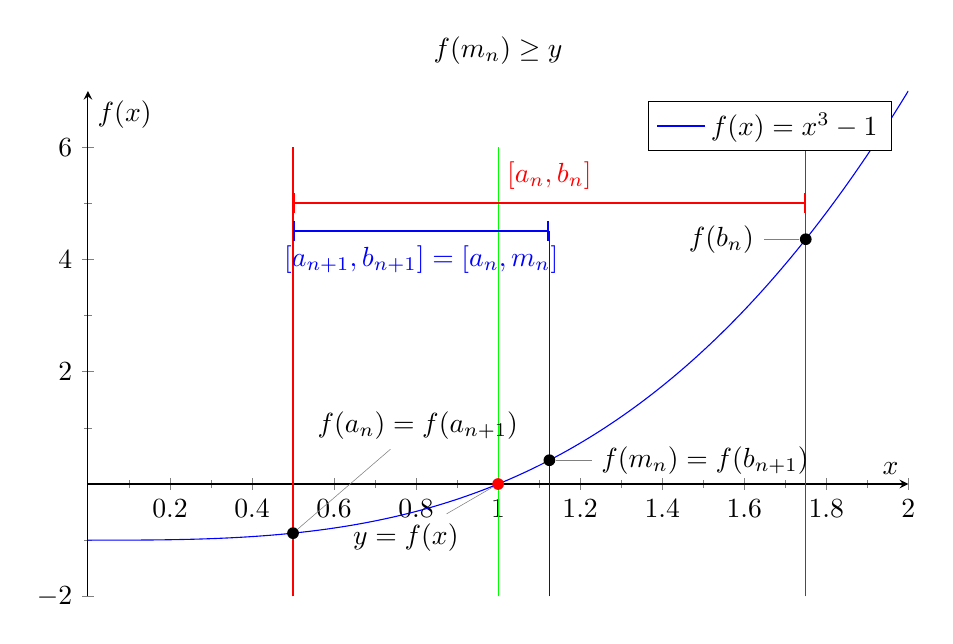
\begin{tikzpicture}
        \tikzset {
            small dot/.style={circle,fill,inner sep=1.5pt}
        }
        \begin{axis}[
            title={$f(m_n) \geq y$},
            xlabel={$x$},
            ylabel={$f(x)$},
            minor tick num=1,
            axis lines=middle,
            xmin=0, xmax=2,
            domain=0:2,
            samples=200,
        ]
            \addplot[
                color=blue
            ]{x^3 - 1};
            \addlegendentry{\(f(x) = {x}^3-1\)}:

            % Vertical lines
            \addplot+[red,mark=none] coordinates {(0.5, -2) (0.5, 6)}; % x = a_0
            \addplot+[red,mark=none] coordinates {(1.75, -2) (1.75, 6)}; % x = b_0
            \addplot+[blue,mark=none] coordinates {(1.125, -2) (1.125, 4.5)}; % x = m_0
            \addplot+[green,mark=none] coordinates {(1, -2) (1, 6)}; % x = y

            % The interval labels
            % [a_n, b_n]
            \draw [red,thick,|-|] (axis cs:0.5,5) -- (axis cs:1.75,5);
            \node[red,align=center] at (axis cs:1.125,5.5) {$[a_n, b_n]$};

            % [a_{n + 1}, b_{n + 1}]
            \draw [blue,thick,|-|] (axis cs:0.5,4.5) -- (axis cs:1.125,4.5);
            \node[blue,align=center] at (axis cs:0.8125,4) {$[a_{n + 1}, b_{n + 1}] = [a_n, m_n]$};

            % Point labels
            \node[pin={[pin distance=1cm]80:{$f(a_n) = f(a_{n + 1})$}},small dot] at (axis cs:0.5,0.5^3 - 1) {};
            \node[pin={180:{$f(b_n)$}},small dot] at (axis cs:1.75,1.75^3 - 1) {};
            \node[pin={0:{$f(m_n) = f(b_{n + 1})$}},small dot] at (axis cs:1.125,1.125^3 - 1) {};
            \node[pin={225:{$y = f(x)$}},small dot,red] at (axis cs:1,1^3 - 1) {};
        \end{axis}
    \end{tikzpicture}
\end{frame}

\begin{frame}
    \frametitle{High-level overview of the proof and the basis for the algorithm}

    Otherwise, if $f(m_n) < y$, i.e., the value of $f$ at the middle of $[a_n, b_n]$ is less than $y = f(x)$ and, conversely,
    thanks to the continuity of $f$, we can assume $m_n < x$, therefore, picking $a_{n + 1} = m_n$, $b_{n + 1} = b_n$ which still preseves the main property: $f(a_{n + 1}) < y < f(b_{n + 1})$. \\~\

    The $[a_{n + 1}, b_{n + 1}] = [m_n, b_n] \subset [a_n, b_n]$ becomes the `right half' of $[a_n, b_n]$.
\end{frame}

\begin{frame}
    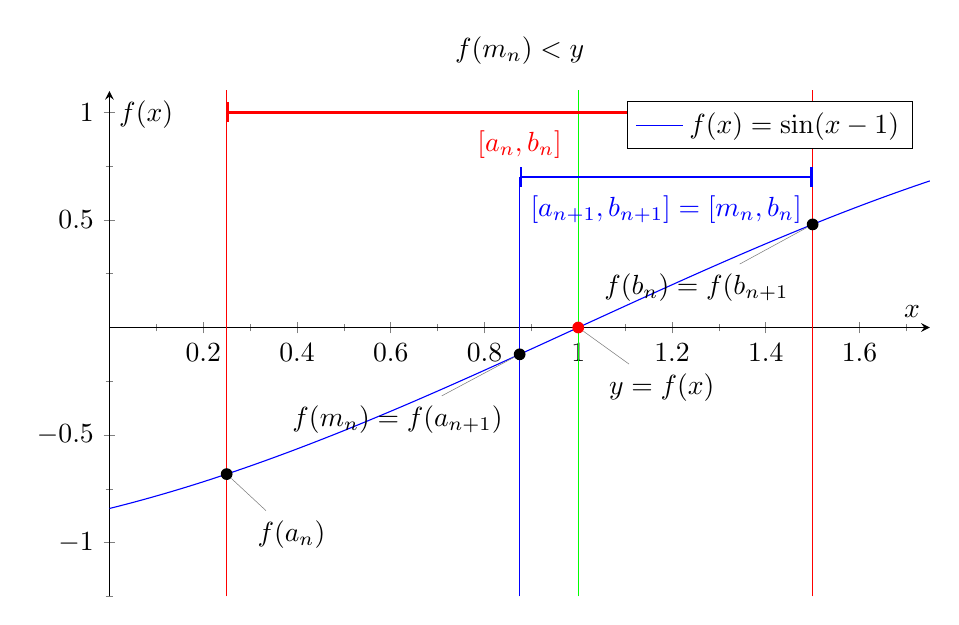
\begin{tikzpicture}
        \tikzset {
            small dot/.style={circle,fill,inner sep=1.5pt}
        }
        \begin{axis}[
            title={$f(m_n) < y$},
            xlabel={$x$},
            ylabel={$f(x)$},
            minor tick num=1,
            axis lines=middle,
            xmin=0, xmax=1.75,
            ymin=-1.25, ymax=1.1,
            domain=0:1.75,
            samples=200,
        ]
            \addplot[
                color=blue,
                trig format=rad,
            ]{sin(x - 1)};
            \addlegendentry{\(f(x) = \sin(x - 1)\)}:

            % Vertical lines
            \addplot+[red,mark=none] coordinates {(0.25, -1.25) (0.25, 1.25)}; % x = a_0
            \addplot+[red,mark=none] coordinates {(1.5, -1.25) (1.5, 1.25)}; % x = b_0
            \addplot+[blue,mark=none] coordinates {(0.875, -1.25) (0.875, 0.7)}; % x = m_0
            \addplot+[green,mark=none] coordinates {(1, -1.25) (1, 1.25)}; % x = y

            % The interval labels
            % [a_n, b_n]
            \draw [red,thick,|-|] (axis cs:0.25,1) -- (axis cs:1.5,1);
            \node[red,align=center] at (axis cs:0.875,0.85) {$[a_n, b_n]$};

            % [a_{n + 1}, b_{n + 1}]
            \draw [blue,thick,|-|] (axis cs:0.875,0.7) -- (axis cs:1.5,0.7);
            \node[blue,align=center] at (axis cs:1.1875,0.55) {$[a_{n + 1}, b_{n + 1}] = [m_n, b_n]$};

            % Point labels
            \node[pin={300:{$f(a_n)$}},small dot] at (axis cs:0.25,-0.6816) {};
            \node[pin={250:{$f(b_n) = f(b_{n + 1}$}},small dot] at (axis cs:1.5,0.4794) {};
            \node[pin={260:{$f(m_n) = f(a_{n + 1})$}},small dot] at (axis cs:0.875,-0.12467) {};
            \node[pin={300:{$y = f(x)$}},small dot,red] at (axis cs:1,0) {};
        \end{axis}
    \end{tikzpicture}
\end{frame}

\section{Bolzano's Theorem}

\begin{frame}
    \frametitle{Bolzano's theorem}

    The extremely relevant collary to the intermediate value theorem is the Bolzano's theorem that is obtained from the intermediate value theorem by considering $y = 0$.

    \begin{corollary}[Bolzano's Theorem]
        Let $f: [a, b] \to \mathbb{R}$ with $f(a) < 0 < f(b)$. \\
        Then $f$ has at least one zero in $(a, b)$, i.e., $\exists x_0 \in (a, b) \colon f(x_0) = 0$.
    \end{corollary}
\end{frame}

\begin{frame}
    \frametitle{The value of $t$}

    The Bolzano's theorem establishes the existance of a solution for an
    important problem of solving the equation $f(x_0) = 0$ for an arbitrary
    continuous function $f$ defined on $[a, b]$ (with the minor constraint $f(a) < 0 < f(b)$ that is easily generalized to $f(a)$ and $f(b)$ having varying signs). \\~\

    Moreover, the proof of the intermediate value theorem hands us an algorithm to find the $x_0$ (or some if there are several) in the interval $(a, b)$.
\end{frame}

\section{Bisection Method Algorithm}

\subsection{The algorithm}

\begin{frame}
    \frametitle{Overview of the bisection method}

    The bisection method makes use of the Bolzano's theorem and the steps of the algorithm can be traced back to the proof of the intermediate value theorem. \\~\

    However, we consider the bisection method for the general case of either $f(a) < 0 < f(b)$ or $f(a) > 0 > f(b)$ and not necessarily just $f(a) < 0 < f(b)$,
    which makes the algorithm a bit more general as compared to the proof discussed above.
\end{frame}

\begin{frame}
    \frametitle{Generalizing the conditions}

    To achieve this generalization we observe that the property being maintained
    by the assignment throught the proof is $f(a) < y < f(b)$ (for $y = 0$:
    $f(a) < 0 < f(b)$) and it is being maintained by assigning the next values
    of $a_n$ and $b_n$ in such a way that does not invalidate the property,
    i.e., picking the appropriate half. \\~\

    More generally, the signs of $f(a)$ and $f(b)$ are maintained. And this
    obersvation also generalizes to the other case of $f(a) > 0 > f(b)$, where
    we want to maintain the signs of $f(a)$ and $f(b)$ by assigning $m$ to
    either $a$ or $b$.
\end{frame}

\begin{frame}
    \frametitle{The algorithm}

    The steps of the algorithm:

    \begin{enumerate}
        \item<1-> Compute $m = \frac{a + b}{2}$ and $f(m)$;
        \item<2-> If $f(m)$ = 0, then we are done: $x_0 = m$;
        \item<3-> Else if $f(a)$ and $f(m)$ have the same sign, i.e., $f(a) \cdot f(m) > 0$, then we set $a = m$ and 
            retain the value of $b$ upholding that $f(a)$ and $f(b)$ have different signs and $x_0 \in (a, b)$ by the Bolzano's theorem;
        \item<4-> Otherwise the $f(a)$ and $f(m)$ have varying signs, we retain the value of $a$ and
            set $b = m$, once again upholding the property that $f(a)$ and $f(b)$ have varying signs and $x_0 \in (a, b)$ by the Bolzano's theorem;
        \item<5-> Repeat the above steps until we have found the precise $x_0$ or the value of $m$ is \emph{close enough} to the actual $x_0$: $b - a < \varepsilon \implies |x_0 - m| < \varepsilon$, more on that in the next slides.
    \end{enumerate}
\end{frame}

\subsection{Approximation Error}

\begin{frame}
    \frametitle{Approximation error}

    As $m_n \to x_0$ as $n \to \infty$, but $x_0$ is actually only attained in $\infty$, and attaining infinity is definitely not feasiable, so we need
    to know when the the value of $m_n$ is \emph{close enough} to the actual value of $x_0$. We can do this by considering the absolute error $|x - m_n|$
    and reducing it to some desired $\varepsilon$. \\~\

    By repeatedly shriking the interval, we can approximate $x_0$ by $m_n$ up to some $\varepsilon$, i.e., $|x_0 - m_n| < \varepsilon$. \\~\
\end{frame}

\begin{frame}
    \frametitle{Approximation error}

    Let's prove the intuitive idea of the distance between the $x_0$ and $m$ being less that the length of the interval $(a_n, b_n)$ in which they are contained. \\~\

    Prove $|x_0 - m_n| < b_n - a_n$.
    \begin{equation}
        \label{x_bounds}
        a_n < x_0 < b_n
    \end{equation}
    by the continuity of $f$ from $f(a_n) < f(x_0) < f(b_n)$
\end{frame}

\begin{frame}
    \frametitle{Approximation error}

    Case 1: $x_0 - m_n \geq 0$

    $$|x_0 - m_n| = x_0 - m_n \overset{(\ref{middle_bounds}, \ref{x_bounds})}{<} b_n - a_n$$

    Case 2: $x_0 - m_n < 0$

    $$|x_0 - m_n| = -x_0 + m_n = m_n - x_0 \overset{(\ref{middle_bounds}, \ref{x_bounds})}{<} b_n - a_n$$

    $$|x_0 - m_n| < b_n - a_n$$

    \qed
\end{frame}

\begin{frame}
    \frametitle{}

    As $|x - m_n| < b_n - a_n$, i.e., $b_n - a_n < \varepsilon \implies |m_n - x| < \varepsilon$, the condition $|x - m_n| < \varepsilon$
    will certainly be satisfied by repeating the procedure while $|b - a| = b - a \geq \varepsilon$.
\end{frame}

\section{Examples}
\subsection{Example 1}

\begin{frame}
    \frametitle{Example 1}

    Consider the function $f \colon [0.5, 2.5] \to \mathbb{R}$, $f(x) = x^3 - 3$ and let's try to find the $x_0$, s.t. $f(x_0) = 0$.
\end{frame}

\begin{frame}
    \frametitle{Example 1: Visualization}

    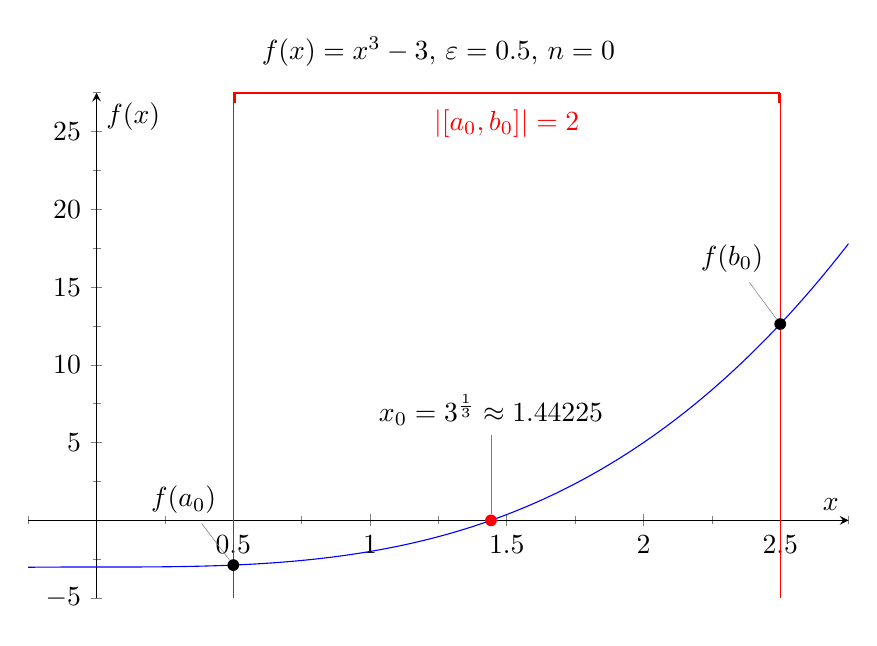
\begin{tikzpicture}
        \tikzset {
            small dot/.style={circle,fill,inner sep=1.5pt}
        }
        \begin{axis}[
            title={$f(x) = x^3 - 3$, $\varepsilon = 0.5$, $n = 0$},
            xlabel={$x$},
            ylabel={$f(x)$},
            minor tick num=1,
            axis lines=middle,
            xmin=-0.25, xmax=2.75,
            domain=-0.25:2.75,
            samples=200,
        ]
            \addplot[
                color=blue
            ]{x^3 - 3};

            \addplot+[red,solid,mark=none] coordinates {(0.5, -5) (0.5, 27.5)};
            \addplot+[red,solid,mark=none] coordinates {(2.5, -5) (2.5, 27.5)};
            \draw [red,thick,|-|] (axis cs:0.5,27.5) -- (axis cs:2.5,27.5);
            \node[red,align=center] at (axis cs:1.5,25.5) {$|[a_0, b_0]| = 2$};
            \node[pin={100:{$f(a_0)$}},small dot] at (axis cs:0.5,-2.875) {};
            \node[pin={100:{$f(b_0)$}},small dot] at (axis cs:2.5,12.625) {};

            \node[pin={[pin distance=1cm]90:{$x_0 = 3^{\frac{1}{3}} \approx 1.44225$}},small dot,red] at (axis cs:1.4422492980957031,0) {};
        \end{axis}
    \end{tikzpicture}
\end{frame}

\begin{frame}
    \frametitle{Example 1: Visualization}

    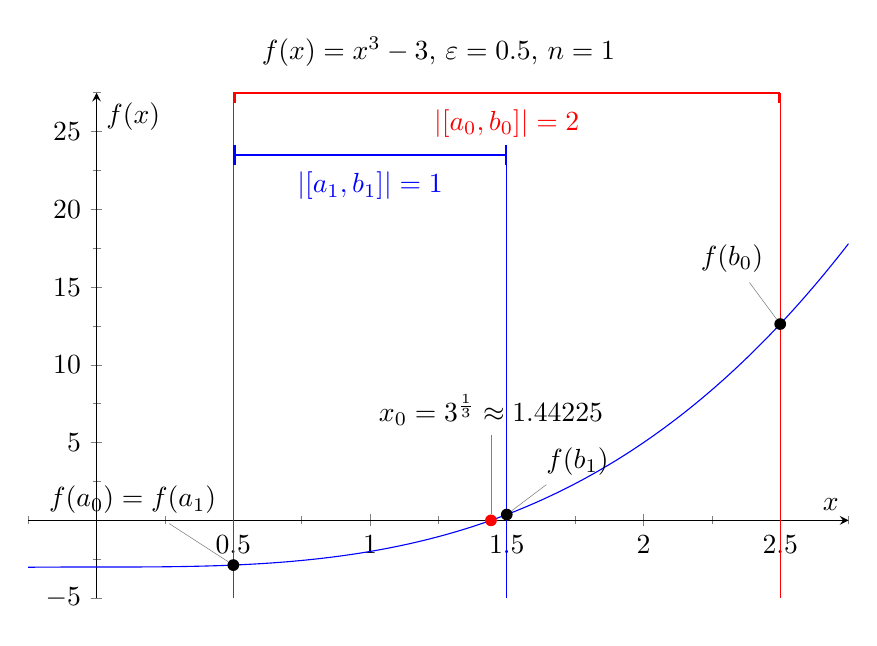
\begin{tikzpicture}
        \tikzset {
            small dot/.style={circle,fill,inner sep=1.5pt}
        }
        \begin{axis}[
            title={$f(x) = x^3 - 3$, $\varepsilon = 0.5$, $n = 1$},
            xlabel={$x$},
            ylabel={$f(x)$},
            minor tick num=1,
            axis lines=middle,
            xmin=-0.25, xmax=2.75,
            domain=-0.25:2.75,
            samples=200,
        ]
            \addplot[
                color=blue
            ]{x^3 - 3};

            \addplot+[red,solid,mark=none] coordinates {(0.5, -5) (0.5, 27.5)};
            \addplot+[red,solid,mark=none] coordinates {(2.5, -5) (2.5, 27.5)};
            \draw [red,thick,|-|] (axis cs:0.5,27.5) -- (axis cs:2.5,27.5);
            \node[red,align=center] at (axis cs:1.5,25.5) {$|[a_0, b_0]| = 2$};
            \node[pin={100:{$f(a_0) = f(a_1)$}},small dot] at (axis cs:0.5,-2.875) {};
            \node[pin={100:{$f(b_0)$}},small dot] at (axis cs:2.5,12.625) {};

            \addplot+[blue,solid,mark=none] coordinates {(1.5, -5) (1.5, 23.5)};
            \draw [blue,thick,|-|] (axis cs:0.5,23.5) -- (axis cs:1.5,23.5);
            \node[blue,align=center] at (axis cs:1.0,21.5) {$|[a_1, b_1]| = 1$};
            \node[pin={45:{$f(b_1)$}},small dot] at (axis cs:1.5,0.375) {};

            \node[pin={[pin distance=1cm]90:{$x_0 = 3^{\frac{1}{3}} \approx 1.44225$}},small dot,red] at (axis cs:1.4422492980957031,0) {};
        \end{axis}
    \end{tikzpicture}
\end{frame}

\begin{frame}
    \frametitle{Example 1: Visualization}

    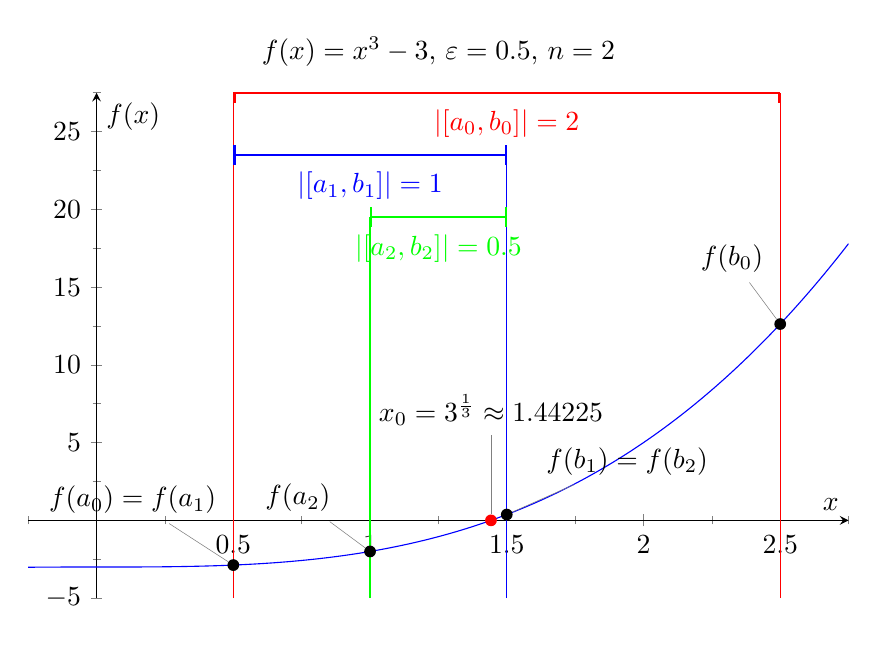
\begin{tikzpicture}
        \tikzset {
            small dot/.style={circle,fill,inner sep=1.5pt}
        }
        \begin{axis}[
            title={$f(x) = x^3 - 3$, $\varepsilon = 0.5$, $n = 2$},
            xlabel={$x$},
            ylabel={$f(x)$},
            minor tick num=1,
            axis lines=middle,
            xmin=-0.25, xmax=2.75,
            domain=-0.25:2.75,
            samples=200,
        ]
            \addplot[
                color=blue
            ]{x^3 - 3};

            \addplot+[red,solid,mark=none] coordinates {(0.5, -5) (0.5, 27.5)};
            \addplot+[red,solid,mark=none] coordinates {(2.5, -5) (2.5, 27.5)};
            \draw [red,thick,|-|] (axis cs:0.5,27.5) -- (axis cs:2.5,27.5);
            \node[red,align=center] at (axis cs:1.5,25.5) {$|[a_0, b_0]| = 2$};
            \node[pin={100:{$f(a_0) = f(a_1)$}},small dot] at (axis cs:0.5,-2.875) {};
            \node[pin={100:{$f(b_0)$}},small dot] at (axis cs:2.5,12.625) {};

            \addplot+[blue,solid,mark=none] coordinates {(1.5, -5) (1.5, 23.5)};
            \draw [blue,thick,|-|] (axis cs:0.5,23.5) -- (axis cs:1.5,23.5);
            \node[blue,align=center] at (axis cs:1.0,21.5) {$|[a_1, b_1]| = 1$};
            \node[pin={45:{$f(b_1) = f(b_2)$}},small dot] at (axis cs:1.5,0.375) {};

            \addplot+[green,solid,mark=none] coordinates {(1.0, -5) (1.0, 19.5)};
            \draw [green,thick,|-|] (axis cs:1.0,19.5) -- (axis cs:1.5,19.5);
            \node[green,align=center] at (axis cs:1.25,17.5) {$|[a_2, b_2]| = 0.5$};
            \node[pin={135:{$f(a_2)$}},small dot] at (axis cs:1.0,-2.0) {};

            \node[pin={[pin distance=1cm]90:{$x_0 = 3^{\frac{1}{3}} \approx 1.44225$}},small dot,red] at (axis cs:1.4422492980957031,0) {};
        \end{axis}
    \end{tikzpicture}
\end{frame}

\begin{frame}
    \frametitle{Example 1: Visualization}

    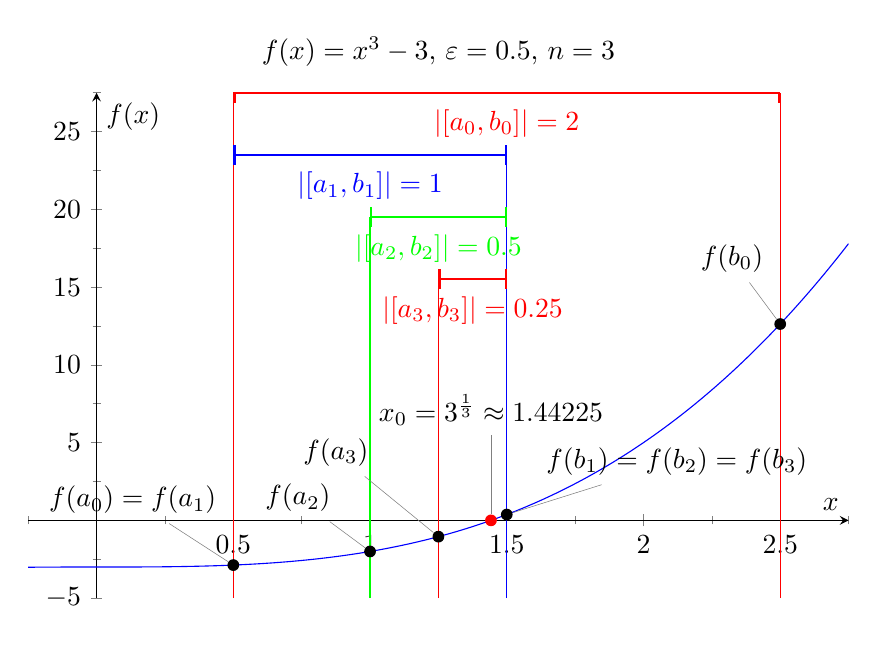
\begin{tikzpicture}
        \tikzset {
            small dot/.style={circle,fill,inner sep=1.5pt}
        }
        \begin{axis}[
            title={$f(x) = x^3 - 3$, $\varepsilon = 0.5$, $n = 3$},
            xlabel={$x$},
            ylabel={$f(x)$},
            minor tick num=1,
            axis lines=middle,
            xmin=-0.25, xmax=2.75,
            domain=-0.25:2.75,
            samples=200,
        ]
            \addplot[
                color=blue
            ]{x^3 - 3};

            \addplot+[red,solid,mark=none] coordinates {(0.5, -5) (0.5, 27.5)};
            \addplot+[red,solid,mark=none] coordinates {(2.5, -5) (2.5, 27.5)};
            \draw [red,thick,|-|] (axis cs:0.5,27.5) -- (axis cs:2.5,27.5);
            \node[red,align=center] at (axis cs:1.5,25.5) {$|[a_0, b_0]| = 2$};
            \node[pin={100:{$f(a_0) = f(a_1)$}},small dot] at (axis cs:0.5,-2.875) {};
            \node[pin={100:{$f(b_0)$}},small dot] at (axis cs:2.5,12.625) {};

            \addplot+[blue,solid,mark=none] coordinates {(1.5, -5) (1.5, 23.5)};
            \draw [blue,thick,|-|] (axis cs:0.5,23.5) -- (axis cs:1.5,23.5);
            \node[blue,align=center] at (axis cs:1.0,21.5) {$|[a_1, b_1]| = 1$};
            \node[pin={45:{$f(b_1) = f(b_2) = f(b_3)$}},small dot] at (axis cs:1.5,0.375) {};

            \addplot+[green,solid,mark=none] coordinates {(1.0, -5) (1.0, 19.5)};
            \draw [green,thick,|-|] (axis cs:1.0,19.5) -- (axis cs:1.5,19.5);
            \node[green,align=center] at (axis cs:1.25,17.5) {$|[a_2, b_2]| = 0.5$};
            \node[pin={135:{$f(a_2)$}},small dot] at (axis cs:1.0,-2.0) {};

            \addplot+[red,solid,mark=none] coordinates {(1.25, -5) (1.25, 15.5)};
            \draw [red,thick,|-|] (axis cs:1.25,15.5) -- (axis cs:1.5,15.5);
            \node[red,align=center] at (axis cs:1.375,13.5) {$|[a_3, b_3]| = 0.25$};
            \node[pin={[pin distance=1cm]135:{$f(a_3)$}},small dot] at (axis cs:1.25,-1.046875) {};

            \node[pin={[pin distance=1cm]90:{$x_0 = 3^{\frac{1}{3}} \approx 1.44225$}},small dot,red] at (axis cs:1.4422492980957031,0) {};
        \end{axis}
    \end{tikzpicture}
\end{frame}

\begin{frame}
    \frametitle{Example 1: Output of the Python program}

    \begin{figure}
        \centering
        \includegraphics[width=0.8\textwidth]{x**3-3,eps=0.5}
        \caption{Output for $f(x) = x^3 - 3$, $[a, b] = [0.5, 2.5]$, $\varepsilon = 0.5$.}
    \end{figure}
\end{frame}

\begin{frame}
    \frametitle{Example 1: Output of the Python program}

    \begin{figure}
        \centering
        \includegraphics[width=0.8\textwidth]{x**3-3,eps=0.001}
        \caption{Output for $f(x) = x^3 - 3$, $[a, b] = [0.5, 2.5]$, $\varepsilon = 0.001$.}
    \end{figure}
\end{frame}

\subsection{Example 2}

\begin{frame}
    \frametitle{Example 2}

    Consider the function $f \colon [0.25, 1.25] \to \mathbb{R}$, $f(x) = \sin(x - 1)$ and let's try to find the $x_0$, s.t. $f(x_0) = 0$.
\end{frame}

\begin{frame}
    \frametitle{Example 2: Visualization}
    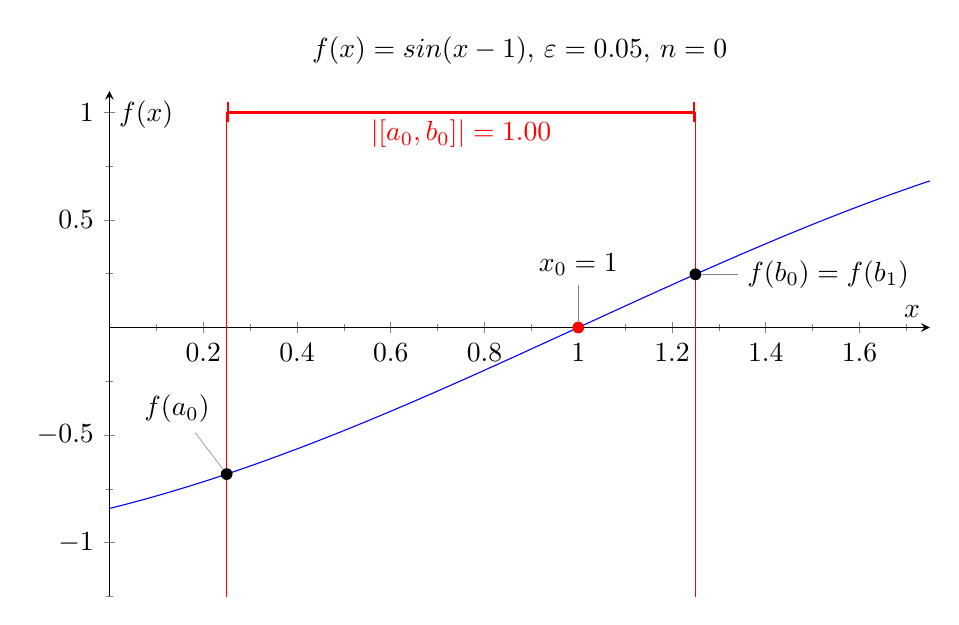
\begin{tikzpicture}
        \tikzset {
            small dot/.style={circle,fill,inner sep=1.5pt}
        }
        \begin{axis}[
            title={$f(x) = sin(x - 1)$, $\varepsilon = 0.05$, $n = 0$},
            xlabel={$x$},
            ylabel={$f(x)$},
            minor tick num=1,
            axis lines=middle,
            xmin=0, xmax=1.75,
            ymin=-1.25, ymax=1.1,
            domain=0:1.75,
            samples=200,
        ]
            \addplot[
                color=blue,
                trig format=rad,
            ]{sin(x - 1)};

            \addplot+[red,solid,mark=none] coordinates {(0.25, -5) (0.25, 1)};
            \addplot+[red,solid,mark=none] coordinates {(1.25, -5) (1.25, 1)};
            \draw [red,thick,|-|] (axis cs:0.25,1) -- (axis cs:1.25,1);
            \node[red,align=center] at (axis cs:0.75,0.9) {$|[a_0, b_0]| = 1.00$};
            \node[pin={100:{$f(a_0)$}},small dot] at (axis cs:0.25,-0.6816387600233341) {};
            \node[pin={0:{$f(b_0) = f(b_1)$}},small dot] at (axis cs:1.25,0.24740395925452294) {};

            \node[pin={90:{$x_0 = 1$}},small dot,red] at (axis cs:1.0,0) {};
        \end{axis}
    \end{tikzpicture}
\end{frame}

\begin{frame}
    \frametitle{Example 2: Visualization}
    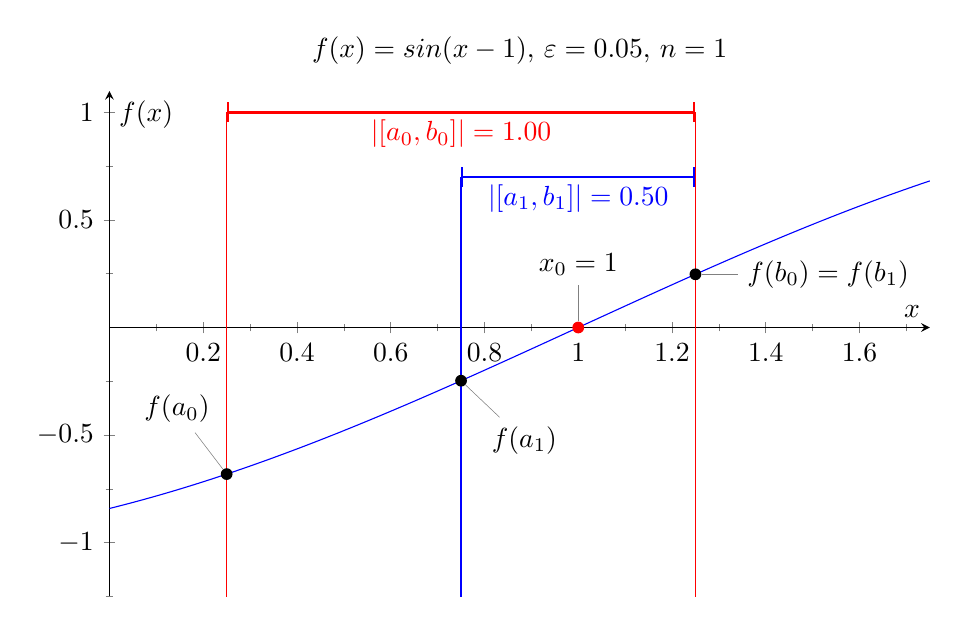
\begin{tikzpicture}
        \tikzset {
            small dot/.style={circle,fill,inner sep=1.5pt}
        }
        \begin{axis}[
            title={$f(x) = sin(x - 1)$, $\varepsilon = 0.05$, $n = 1$},
            xlabel={$x$},
            ylabel={$f(x)$},
            minor tick num=1,
            axis lines=middle,
            xmin=0, xmax=1.75,
            ymin=-1.25, ymax=1.1,
            domain=0:1.75,
            samples=200,
        ]
            \addplot[
                color=blue,
                trig format=rad,
            ]{sin(x - 1)};

            \addplot+[red,solid,mark=none] coordinates {(0.25, -5) (0.25, 1)};
            \addplot+[red,solid,mark=none] coordinates {(1.25, -5) (1.25, 1)};
            \draw [red,thick,|-|] (axis cs:0.25,1) -- (axis cs:1.25,1);
            \node[red,align=center] at (axis cs:0.75,0.9) {$|[a_0, b_0]| = 1.00$};
            \node[pin={100:{$f(a_0)$}},small dot] at (axis cs:0.25,-0.6816387600233341) {};
            \node[pin={0:{$f(b_0) = f(b_1)$}},small dot] at (axis cs:1.25,0.24740395925452294) {};

            \addplot+[blue,solid,mark=none] coordinates {(0.75, -5) (0.75, 0.7)};
            \draw [blue,thick,|-|] (axis cs:0.75,0.7) -- (axis cs:1.25,0.7);
            \node[blue,align=center] at (axis cs:1.0,0.6) {$|[a_1, b_1]| = 0.50$};
            \node[pin={-60:{$f(a_1)$}},small dot] at (axis cs:0.75,-0.24740395925452294) {};

            \node[pin={90:{$x_0 = 1$}},small dot,red] at (axis cs:1.0,0) {};
        \end{axis}
    \end{tikzpicture}
\end{frame}

\begin{frame}
    \frametitle{Example 2: Output of the Python program}

    \begin{figure}
        \centering
        \includegraphics[width=0.8\textwidth]{sin(x-1),eps=0.05}
        \caption{Output for $f(x) = sin(x - 1)$, $[a, b] = [0.25, 1.25]$, $\varepsilon = 0.05$.}
    \end{figure}
\end{frame}

\end{document}
